% !TeX root = ../main.tex

\chapter{结果结论}
图\ref{EEE}和图\ref{UUU}分别显示了莫比乌斯岛周围的电场、电势分布状况。
\begin{figure}[h]
  \centering
  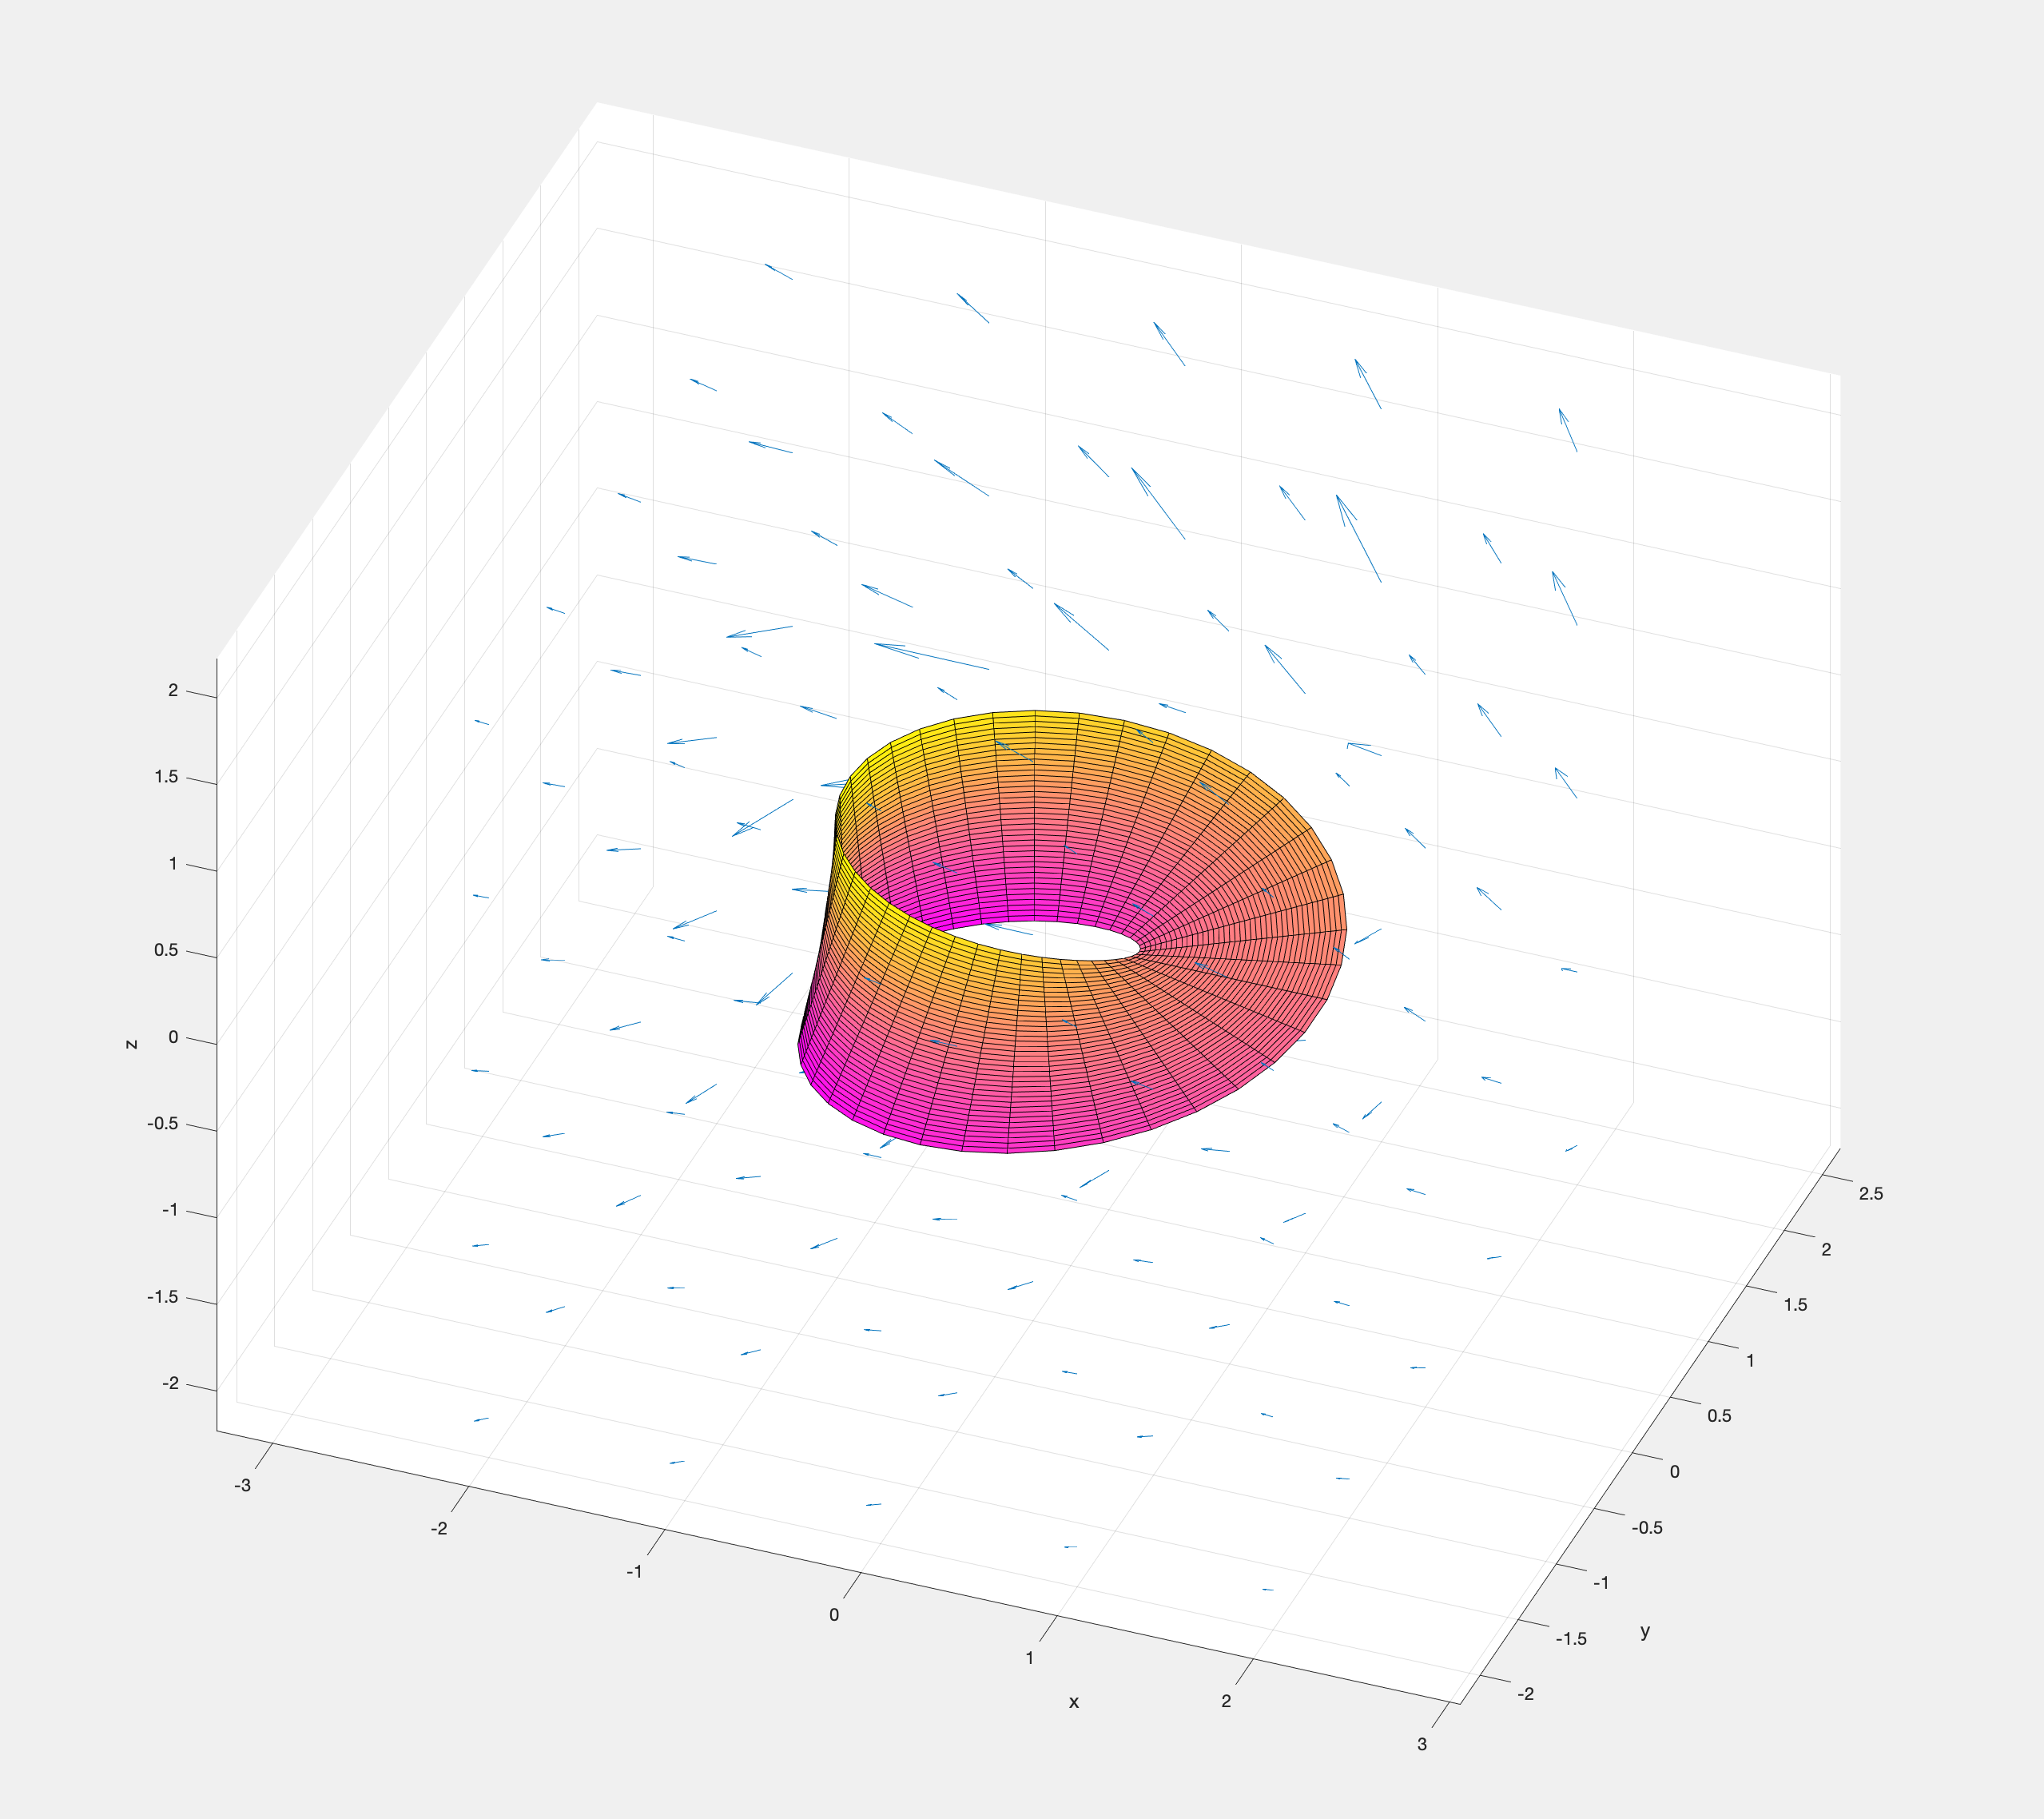
\includegraphics[width=0.7\textwidth]{E.png}
  \caption{莫比乌斯带周围电场的分布}\label{EEE}
  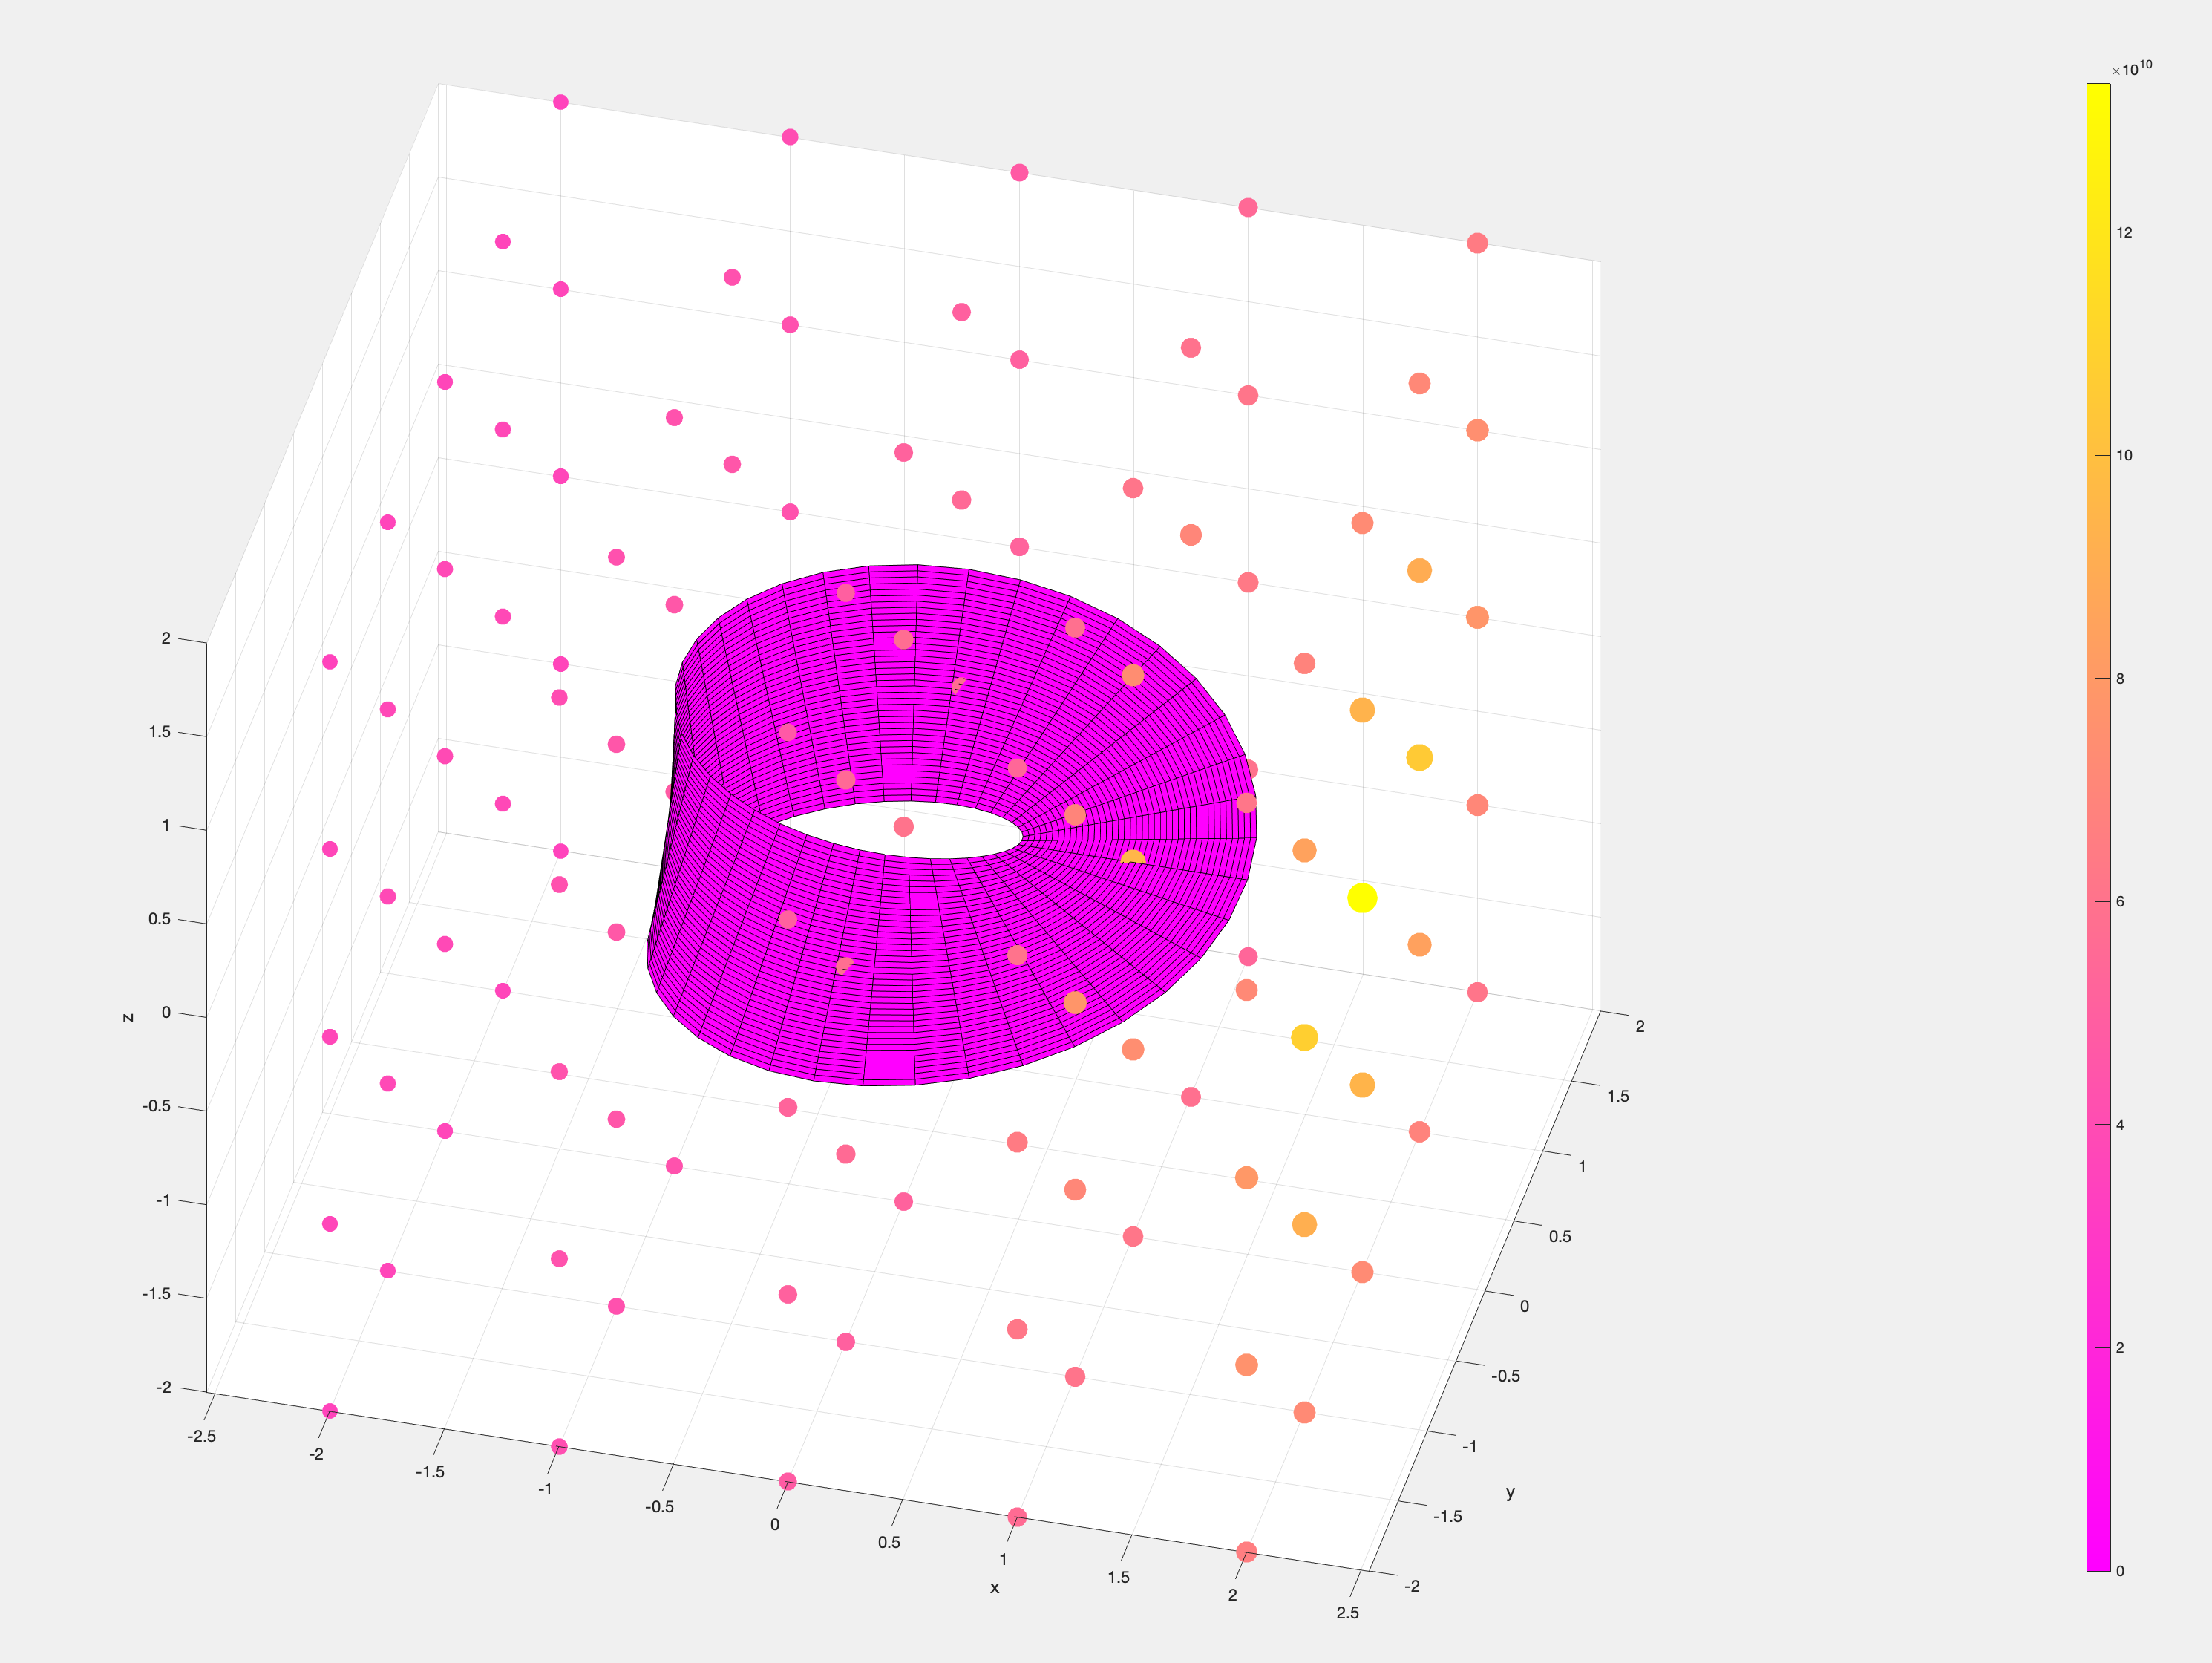
\includegraphics[width=0.7\textwidth]{U.png}
  \caption{莫比乌斯带周围电势的分布}\label{UUU}
\end{figure}

从图中可以看出,靠近莫比乌斯带面的地方,电场强度矢量基本垂直于该面切平面,与法向量平行。
此外,y坐标大的地方,电场强度更大;距中心圆点相同距离的点x坐标大的,电势更高。
\newpage
\begin{thebibliography}{4}%不使用BibTeX的方法;99意为参考文献的最大数值为99个,这个数可以自己设置
    \bibitem{ref0}百度百科. 莫比乌斯带[DB/OL]. (2022-11-21)[2022-12-11]. https://baike.baidu.com/item/莫比乌斯带/4457881
    \bibitem{ref00}百度文库. 莫比乌斯带——精选推荐[DB/OL]. [2022-12-11]. https://wenku.baidu.com/view/6823a462ae02de\\80d4d8d15abe23482fb4da02ca.html?$\_$wkts$\_$=1670857341735\&bdQuery=莫比乌斯带带电
    \bibitem{ref01}百度百科. 电场叠加原理[DB/OL]. (2022-11-21)[2022-12-11]. https://baike.baidu.com/item/电场叠加原理/846636
    \bibitem{ref1}知乎. 莫比乌斯带的参数方程是怎么来的?它又为什么没有方向呢?[EB/OL]. (2019-07-30)[2022-12-11]. https://zhuanlan.zhihu.com/p/75237170
    \bibitem{ref2}叶邦角. 电磁学[M]. 第2版. 合肥: 中国科学技术大学出版社, 2018: 28-47.
\end{thebibliography}